\section{Results}\label{sec:results}

% describe data
We apply our method to a set of mock data, in a first run on the
spherical models for the Gaia challenge by Walker. They consist of
dynamical tracer populations with density distribution

\begin{equation}
    \nu_*(r) = \nu_0\left(\frac{r}{r_*}\right)^{-\gamma_*} \left[1+\left(\frac{r}{r_*}\right)^{\alpha_*}\right]^{(\gamma_*-\beta_*)/\alpha_*}
\end{equation}

inside dark matter halos of the form

\begin{equation}
    \rho_{\text{DM}} = \rho_0\left(\frac{r}{r_{\text{DM}}}\right)^{-\gamma_{\text{DM}}}\left[1+\left(\frac{r}{r_{\text{DM}}}\right)^{\alpha_{\text{DM}}}\right]^{(\gamma_{\text{DM}}-\beta_{\text{DM}})/\alpha_{\text{DM}}}
\end{equation}

with scale radii $r_*, r_\text{DM}$, central slopes of $\gamma_*,
\gamma_{\text{DM}}$, transition parameters
$\beta_*,\beta_{\text{DM}}$, and outer slopes $\alpha_*,
\alpha_{\text{DM}}$.

The anisotropy follows the functional form of \citet{Osipkov1979} and
\citet{Merritt1985},

\begin{equation}
    \beta(r)=1-\frac{\sigma_\theta^2}{\sigma_r^2} = \frac{r^2}{r^2+r_a^2}.
\end{equation}

with scale radius $r_a$, turning over from nearly isotropic at $r\to
0$ to radially biased at $r_*=r_a$.

Of these distributions, finite samplings are taken and converted to
mock observational data including observational parameters like
spectral indices, systemic velocities, proper motions, and binary
motions.

\subsection{Cusps and Cores}

Applied on a profile with a cusp in the DM density profile,
$\gamma_{DM}=1$, our method reproduces the density profile
(fig. \ref{fig:cusp1pop}). The further characteristics of the particular
mock model are stellar central density slope $\gamma_{*,1}=0.1,
\gamma_{*,2}=0.1$, stellar turnover slopes
$\beta_{*,1}=\beta_{*,2}=5$, stellar characteristic radii
$r_{*,1}=100\pc, r_{*,2}=500\pc$, and anisotropy scale radii
$r_{a,1}=r_{a,2}=1.0$. We analyze the data with all tracer particles
in one population only first. This population shows a projected tracer
half-light radius of $R_{1/2}=125\pc$.

\begin{figure*}
    \begin{center}
        \hspace{-7mm}
        \includegraphics[width=0.3\textwidth]{fig/prof_1_pop_cusp/prof_rho_0.pdf}
        \includegraphics[width=0.3\textwidth]{fig/prof_1_pop_cusp/prof_nr_0.pdf}
        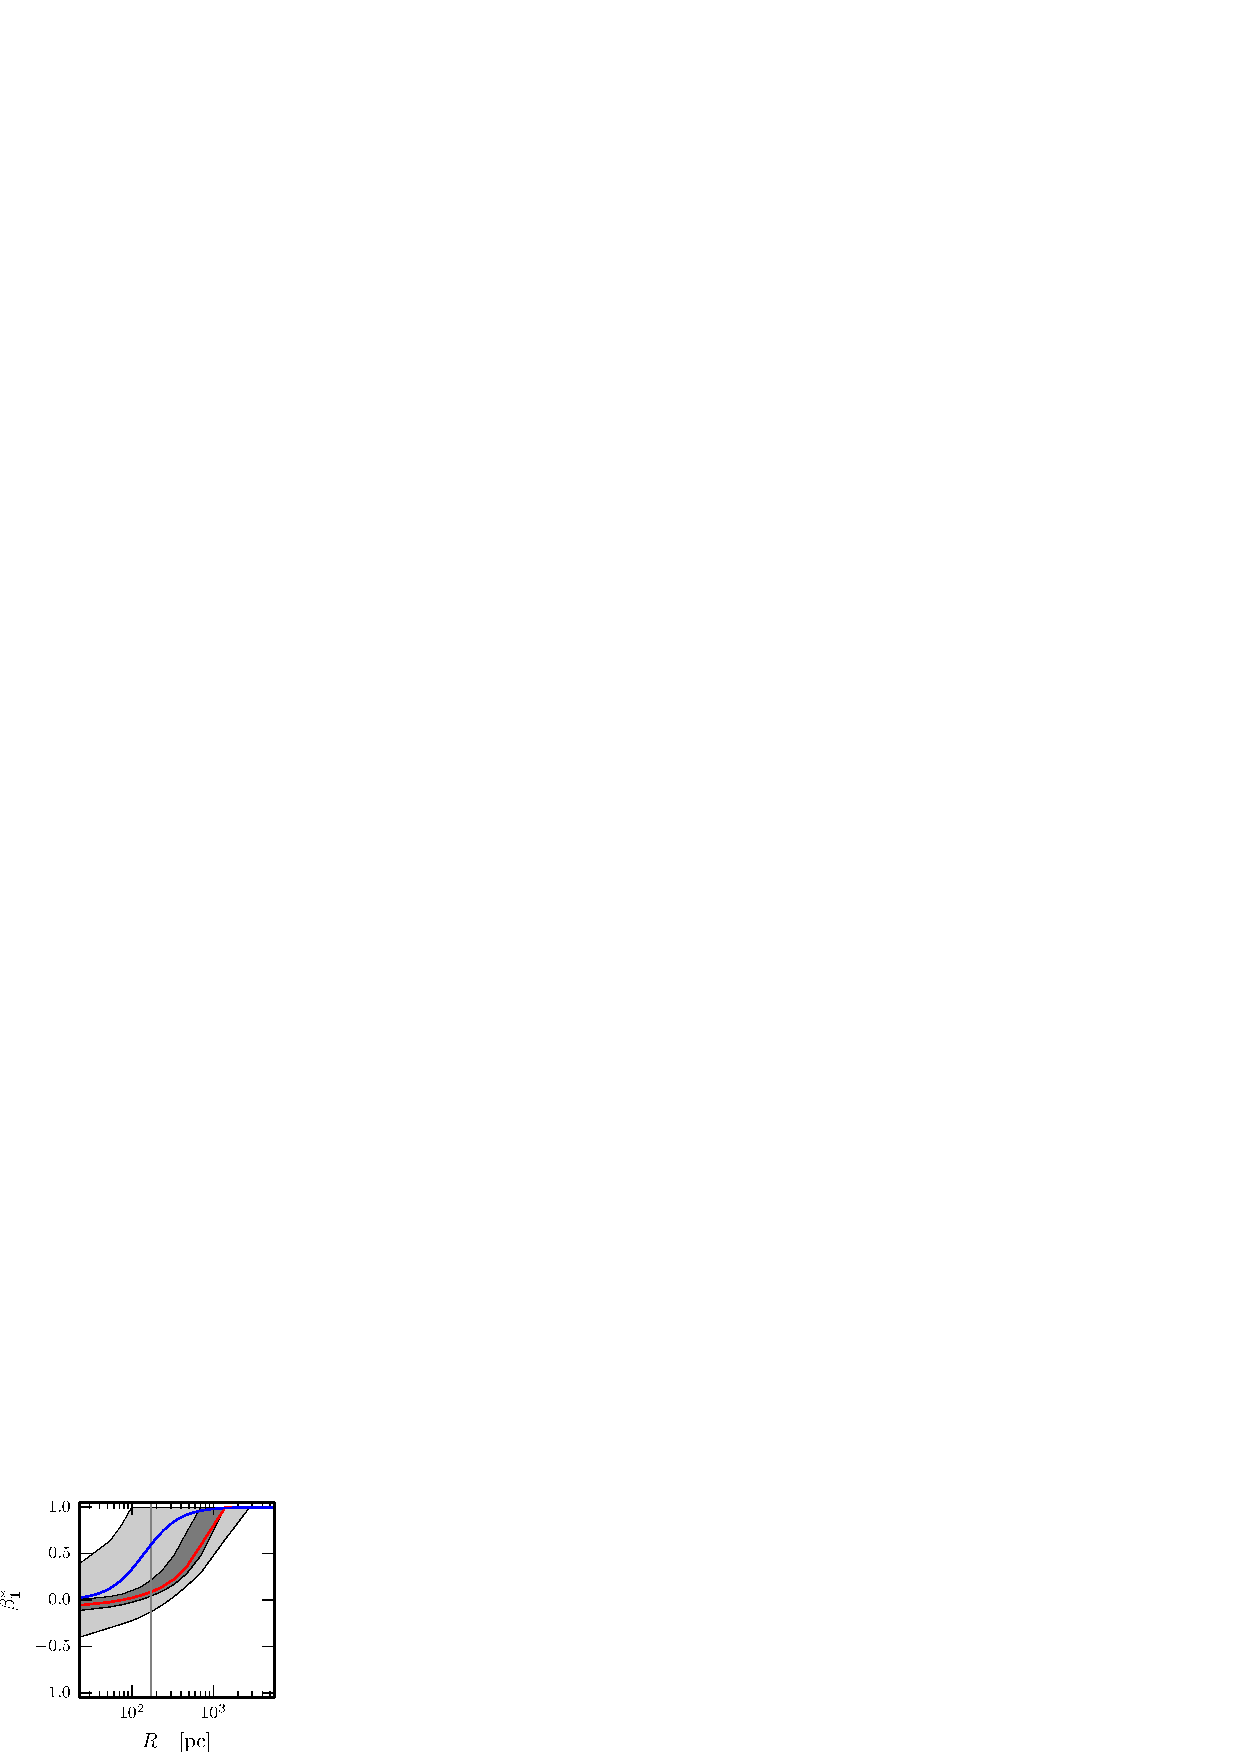
\includegraphics[width=0.3\textwidth]{fig/prof_1_pop_cusp/prof_betastar_1.png}
        \caption{Reconstructed density, density slope, and velocity
          anisotropy of a cusped model (red shows median, shaded areas
          are 68 and 95 percentiles) for $10^4$ tracer particles, for
          $3\cdot10^5$ models. The blue curve shows the underlying
          theoretical model. The half-light radius of all stellar
          tracer particles is depicted as gray vertical line.}
        \label{fig:cusp1pop}
    \end{center}
\end{figure*}

The shown plots depict the 95 and 68 confidence level (light and dark
shaded areas) and the median of all accepted models. The number of
models is equal to the number of live points in MultiNest, and is set
to twice the number of dimensions, $2\cdot N_{\rm dim}$.

% nu and sigma: fit to data
The reconstructed profiles for tracer surface density $\Sigma(r)$ and
velocity dispersion $\siglos(r)$ are shown in fig. \ref{fig:Sigsiglos1pop}.

\begin{figure*}
    \begin{center}
        \hspace{-7mm}
        \includegraphics[width=0.3\textwidth]{fig/prof_1_pop_cusp/prof_Sig_1.pdf}
        \includegraphics[width=0.3\textwidth]{fig/prof_1_pop_cusp/prof_sig_1.pdf}
        \caption{\label{fig:Sigsiglos1pop} Tracer surface density profile
          $\Sigma(r)$, normalized to 1 at $r_{1/2}$ and velocity
          dispersion profile $\siglos(r)$ for the stellar components
          in the cusped profile of fig. \ref{fig:cusp1pop}.}
    \end{center}
\end{figure*}

The original data is given as a blue shaded region. $\chi^2$ is
calculated from the difference between each model's $\Sigma(r)$ and
$\sigma_p(r)$, thus the fact that most models are consistent within
errors to the data is expected from the low $\chi^2 \leq5$ found after
some 1000 iterations.

% Introducing $\kappa_i$ in the $\chi^2$ did \TODO{not?} result in a
% change of behavior for the velocity anisotropy parameter.

\TODO{observations for kurtosis}
\TODO{link to Tom's papers: kappa does not resolve density/anisotropy degeneracy,  Virial Shape Parameters do}
\TODO{better/worse fitting of density}

\subsection{Two populations}
The same mock dwarf is analyzed with a model where both populations of
tracer particles are accounted for. This is done in the following
manner: Each particle in the mock dataset has a number identifying it
as a member of population 1, 2, or background. For the plot
\ref{fig:cusp2pop}, we used this information directly.

\begin{figure*}
    \begin{center}
        \hspace{-7mm}
        \includegraphics[width=0.3\textwidth]{fig/prof_2_pop_cusp/prof_rho_0.pdf}
        \includegraphics[width=0.3\textwidth]{fig/prof_2_pop_cusp/prof_nr_0.pdf}
        \caption{Reconstructed density and density slope for the same
          cusped model (red shows median, shaded areas are 68 and 95
          percentiles) for $2\cdot 5000$ tracer particles, for
          $3\cdot10^5$ models. The blue curve shows the underlying
          theoretical model. The half-light radii of the two
          populations of tracer particles is depicted as gray vertical
          lines.}
        \label{fig:cusp2pop}
    \end{center}
\end{figure*}

For real data, we will use a splitting based on metallicity. It has
been shown for several dwarfs (\TODO{cite Walker}) that two or more
dynamically distinct populations (\TODO{what does this mean? how can
we tell one star to be in the right population?}) of stars can be
extracted via their metallicity content.

This is achieved by using a separate Markov Chain Monte Carlo
method. The overall metallicity distribution is represented by a sum
of two Gaussians with means $\mu_{1,2}$ and widths $\sigma_{1,2}$, and
each stellar tracer with metallicity $M$ is assigned a population
based on the likelihood of its metallicity belonging to said
population. The process is repeated to marginalize over the means and
widths of the metallicity distributions. A sample splitting result is
shown in fig. \ref{fig:pymcmetal}.

\begin{figure}
    \begin{center}
        \hspace{-7mm}
        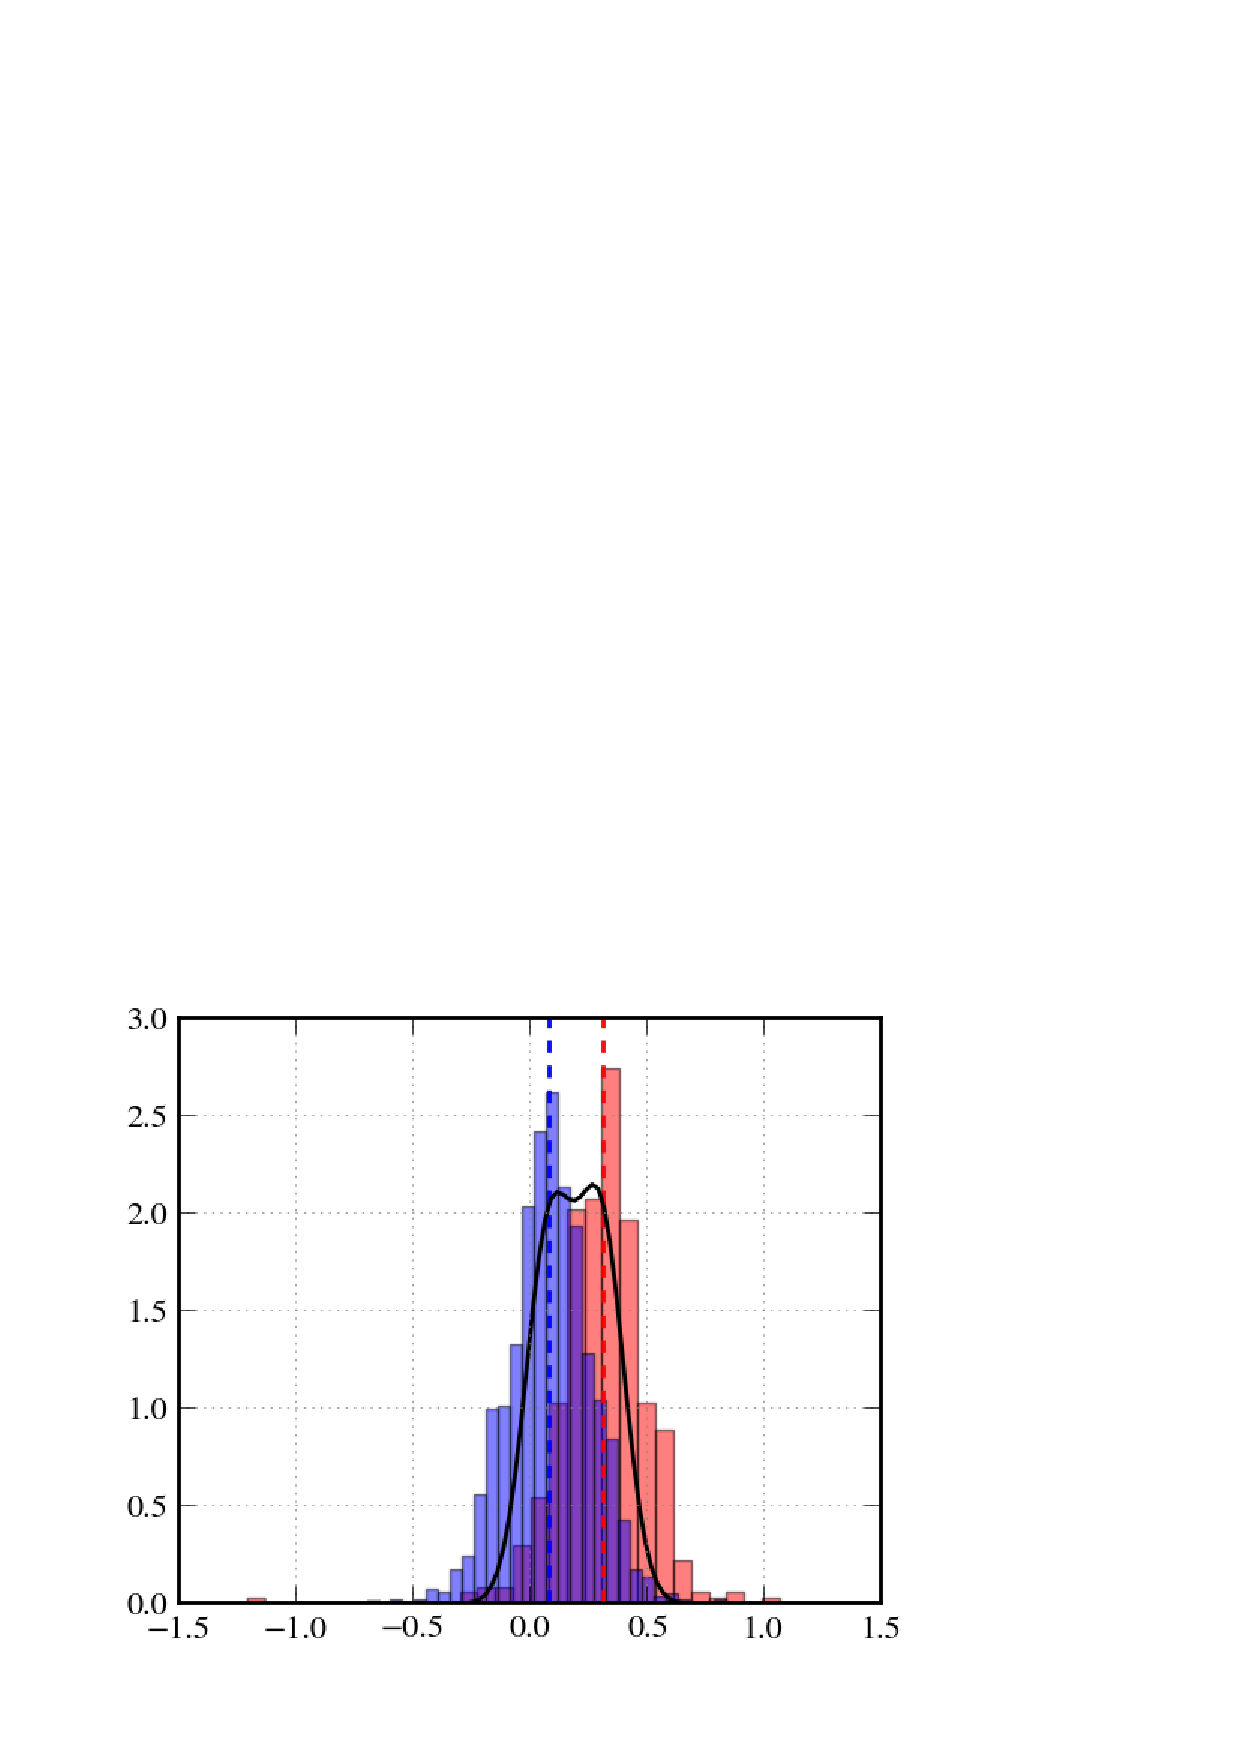
\includegraphics[width=0.5\textwidth]{fig/pymcmetals.png}
        \caption{Reconstruction of two populations from mock data. The
          underlying metallicity distributions are shown as red and
          blue histograms. The retrieved centers of the Gaussians are
          shown as vertical lines, and the reconstructed metallicity
          distribution is depicted as black line.}
        \label{fig:pymcmetal}
    \end{center}
\end{figure}

\TODO{priors} \TODO{3 populations?}

\subsection{Cored Model}
For a cored profile, with $\gamma_{\rm DM}=0$, we get the results in
fig. \ref{fig:core}.

\begin{figure*}
    \begin{center}
        \hspace{-7mm}
        % \includegraphics[width=0.3\textwidth]{fig/prof_2_pops_core/prof_rho_0.pdf}
        % \includegraphics[width=0.3\textwidth]{fig/prof_2_pops_core/prof_rho_0.pdf}
        \caption{A cored profile: Reconstructed mass of the MCMC model
          (red shows median, shaded areas are 68 and 90 percentiles)
          for $10^4$ tracer particles based on $3\cdot10^5$ sampled
          models. The blue curve shows the underlying theoretical
          model.}
        \label{fig:core}
    \end{center}
\end{figure*}


\subsection{Triaxial mock data}
To test the dependency of {\sc Gravlite} on the assumption of
spherical symmetry, we employ it on slightly triaxial mock dwarf
galaxies.

The models were generated with the Made2Measure algorithm of
\cite{Dehnen2009} and are tailored to follow a similar profile to the
profiles specified above for the dwarf galaxies. They show a density
profile of

\begin{equation}
    \rho(r)=\frac{\rho_S}{\left(\frac{r}{r_S}\right)^\gamma\left(1+\left(\frac{r}{r_S}\right)^{1/\alpha}\right)^{\alpha(\beta-\gamma)}}
\end{equation}

with radius $r$, scale radius $r_S=1.5\kpc$, $\alpha=1$,
$\beta=4$. For the cusped profiles we have an inner logarithmic slope
of $\gamma=1$, scale density $\rho_S=5.522\cdot 10^7M_\odot/\kpc^3$,
and $M_{\tot}=1.171\cdot10^9M_\odot$, while for the cored one we have
$\gamma=0.23$, $\rho_S=1.177\cdot10^8M_\odot$,
$M_{\tot}=1.802\cdot10^9M_\odot$. The axis ratios are $b/a=0.8$ and
$c/a=0.6$. The stars have negligible mass and follow the same
functional form in the density profile as dark matter, with
$\alpha=0.34, \beta=5.92, \gamma=0.23, r_S=0.81\kpc$.

The velocity anisotropy of the stellar part is calculated via

\begin{equation}
    \beta(r)=\frac{r_{s,\beta}^\eta \beta_0+r^\eta \beta_\infty}{r^\eta+r_{s,\beta}^\eta},
\end{equation}

with $r_{s,\beta}=0.81\kpc$, $\beta_0=0$, $\beta_\infty=0.5$ and
$\eta=0.5$, going from isotropic to radially anisotropic with
increasing radius.

\begin{figure*}
    \begin{center}
        \hspace{-7mm}
        \includegraphics[width=0.3\textwidth]{fig/prof_1_pop_triax/prof_rho_0.pdf}
        \includegraphics[width=0.3\textwidth]{fig/prof_1_pop_triax/prof_nr_0.pdf}
        \caption{Density profile of a triaxial mock dwarf, for which
          the line of sight is inclined with 45 degrees with respect
          to all axes. The vertical line indicates the half-light
          radius at 640pc.}
        \label{fig:triax}
    \end{center}
\end{figure*}

The retrieved density profile (fig. \ref{fig:triax}) recaptures the
density inside the half-light radius, but constantly overestimates it
at $r>r_{1/2}$. This is partly due to projection effects, as the
underlying density profile in blue is calculated for spherically
averaged density decrease.
